% !TEX root = ../Poissons.tex

\section{Combinatorics of iterated diagonals}

\subsection{Combinatorics of generically translated copies of the braid arrangement}
\label{sec:kBraidArrangement}

\subsubsection{Recollection on hyperplane arrangements}
\label{subsec:arrangements}

We first briefly recall classical results on the combinatorics of affine hyperplane arrangements, in particular the enumerative connection between their intersection posets and their face lattices due to T.~Zaslavsky~\cite{Zaslavsky}.

\begin{definition}
A (finite affine real) \defn{hyperplane arrangement} is a finite set~$\arrangement$ of affine hyperplanes in~$\R^d$.
\end{definition}

\begin{definition}
A \defn{region} of~$\arrangement$ is a connected component of~$\R^d \ssm \bigcup_{H \in \arrangement} H$.
A \defn{face} of~$\arrangement$ is the intersection of the closure of a region of~$\arrangement$ with an hyperplane of~$\arrangement$.
The \defn{face poset} of~$\arrangement$ is the poset~$\facePoset$ of faces of~$\arrangement$ ordered by inclusion.
The \defn{$f$-polynomial}~$\fPol$ and \defn{$b$-polynomial}~$\bPol$ of~$\arrangement$ are the polynomial
\[
\fPol \eqdef \sum_{k = 0}^d f_k(\arrangement) \, x^k
\qquad\text{and}\qquad
\bPol \eqdef \sum_{k = 0}^d b_k(\arrangement) \, x^k
\]
where~$f_k(\arrangement)$ denotes the number of $k$-dimensional faces of~$\arrangement$, while~$b_k(\arrangement)$ denotes the number of bounded $k$-dimensional faces of~$\arrangement$.
\end{definition}

\begin{definition}
A \defn{flat} of~$\arrangement$ is a non-empty affine subspace of~$\R^d$ that can be obtained as the intersection of some hyperplanes of~$\arrangement$.
The \defn{flat poset} of~$\arrangement$ is poset~$\flatPoset$ of flats of~$\arrangement$ ordered by reverse inclusion.
\end{definition}

\begin{definition}
\label{def:MobiusPolynomial}
%The \defn{characteristic polynomial}~$\chi_{\arrangement}(y)$ and the \defn{M\"obius polynomial}~$\mu_{\arrangement}(x,y)$ are the polynomials respectively defined by
%\[
%\charPol \eqdef \sum_{G \in \flatPoset} \mu_{\flatPoset}(\R^d, G) \, y^{\dim(G)}
%\quad\text{and}\quad
%\mobPol \eqdef \sum_{F \le G \in \flatPoset} \mu_{\flatPoset}(F,G) \, x^{\dim(F)} \, y^{\dim(G)}
%\]
The \defn{M\"obius polynomial}~$\mu_{\arrangement}(x,y)$ is the polynomial defined by
\[
\mobPol \eqdef \sum_{F \le G} \mu_{\flatPoset}(F,G) \, x^{\dim(F)} \, y^{\dim(G)},
\]
where~$F \le G$ ranges over all intervals of the flat poset~$\flatPoset$, and~$\mu_{\flatPoset}(F,G)$ denotes the \defn{M\"obius function} on the flat poset~$\flatPoset$ defined as usual by
\[
\mu_{\flatPoset}(F, F) = 1
\qquad\text{and}\qquad
\sum_{F \le G \le H} \mu_{\flatPoset}(F,G) = 0
\]
for all~$F, G, H \in \flatPoset$.
\end{definition}

\begin{remark}
Two observations on \cref{def:MobiusPolynomial}:
\begin{itemize}
\item The coefficient of~$x^d$ in the M\"obius polynomial~$\mobPol$ gives the more classical \defn{characteristic polynomial}
\[
\charPol \eqdef [x^d] \, \mobPol = \sum_G \mu_{\flatPoset}(\R^d,G) \, y^{\dim(G)}.
\]
\item Our definition of the M\"obius polynomial slightly differs from that of \cite{Zaslavsky} as we use the dimension of~$F$ instead of its codimension, in order for the next statement to be slightly simpler.
\end{itemize}
\end{remark}

\begin{theorem}[{\cite[Thm.~A]{Zaslavsky}}]
\label{thm:Zaslavsky}
The $f$-polynomial, the $b$-polynomial, and the M\"obius polynomial of an arrangement~$\arrangement$ are related by
\[
\fPol = \mobPol[\arrangement][-x][-1]
\qquad\text{and}\qquad
\bPol = \mobPol[\arrangement][-x][1].
\]
\end{theorem}

\begin{example}
For the arrangement~$\arrangement$ of $5$ hyperplanes of \cref{fig:arrangement}, we have
\[
\mobPol = x^2y^2 - 5x^2y + 6x^2 + 5xy - 10x + 4
\]
so that
\begin{align*}
\fPol & = \mobPol[\arrangement][-x][-1] = 12 \, x^2 + 15 \, x + 4 \\
\text{and}\qquad
\bPol & = \mobPol[\arrangement][-x][1] = 2 \, x^2 + 5 \, x + 4.
\end{align*}
%
\begin{figure}
%	\begin{overpic}[scale=.9]{intersectionPoset}
%		\put(72.5, -2){$1$}
%		\put(51, 10){$-1$}
%		\put(61, 10){$-1$}
%		\put(71, 10){$-1$}
%		\put(82, 10){$-1$}
%		\put(94, 10){$-1$}
%		\put(51.5, 32){$2$}
%		\put(66, 32){$1$}
%		\put(80, 32){$1$}
%		\put(93.5, 32){$2$}
%	\end{overpic}
%	\caption{A hyperplane arrangement (left) and its intersection poset with its M\"obius function (right).}
	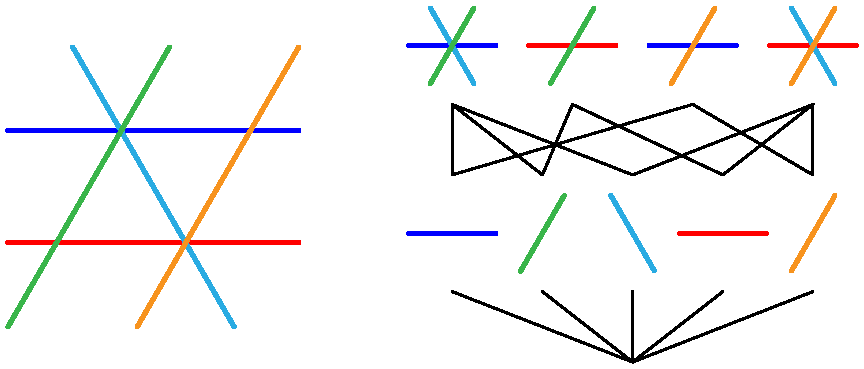
\includegraphics[scale=.9]{intersectionPoset}
	\caption{A hyperplane arrangement (left) and its intersection poset (right).}
	\label{fig:arrangement}
\end{figure}
\end{example}

\subsubsection{The $(\ell,n)$-braid arrrangement}
\label{subsec:lnBraidArrangement}

We now focus on the following specific hyperplane arrangements, illustrated in \cref{fig:lBraidArrangements}, and whose face numbers are given in \cref{table:fvectorlBraidArrangements}.

\begin{figure}
	\centerline{
	\begin{tabular}{c@{\hspace{.7cm}}c@{\hspace{.7cm}}c@{\hspace{.7cm}}c}
		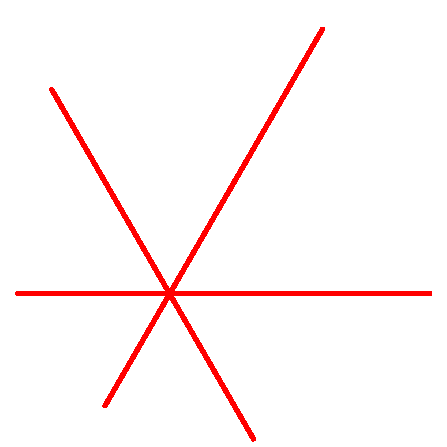
\includegraphics[scale=.4]{lBraidArrangement1}
		&
		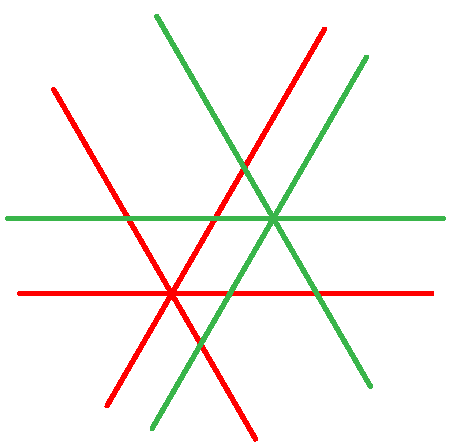
\includegraphics[scale=.4]{lBraidArrangement2}
		&
		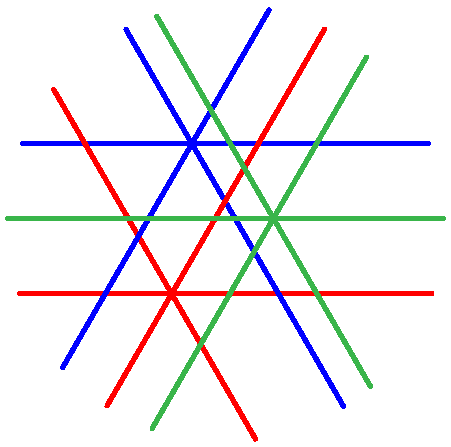
\includegraphics[scale=.4]{lBraidArrangement3}
		&
		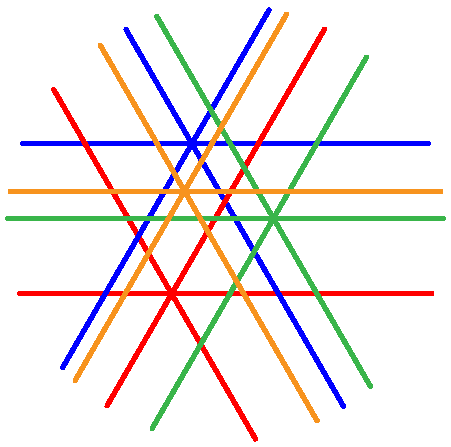
\includegraphics[scale=.4]{lBraidArrangement4}
		\\
		$\ell = 1$ & $\ell = 2$ & $\ell = 3$ & $\ell = 4$
	\end{tabular}
	}
	\caption{The $(\ell,3)$-braid arrangements for~$\ell \in [4]$.}
	\label{fig:lBraidArrangements}
\end{figure}

\begin{table}
\centerline{
	\begin{tabular}{c@{\hspace{.7cm}}c}
		\begin{tabular}[t]{c|cccc|c}
			$n \backslash k$ & $0$ & $1$ & $2$ & $3$ & $\Sigma$ \\
			\hline
			$1$ & $1$ &&&& $1$ \\
			$2$ & $2$ & $1$ &&& $3$ \\
			$3$ & $6$ & $6$ & $1$ && $13$ \\
			$4$ & $24$ & $36$ & $14$ & $1$ & $75$
		\end{tabular}
		&
		\begin{tabular}[t]{c|cccc|c}
			$n \backslash k$ & $0$ & $1$ & $2$ & $3$ & $\Sigma$ \\
			\hline
			$1$ & $1$ &&&& $1$ \\
			$2$ & $3$ & $2$ &&& $5$ \\
			$3$ & $17$ & $24$ & $8$ && $49$ \\
			$4$ & $149$ & $324$ & $226$ & $50$ & $749$
		\end{tabular}
		\\[2cm]
		\begin{tabular}[t]{c|cccc|c}
			$n \backslash k$ & $0$ & $1$ & $2$ & $3$ & $\Sigma$ \\
			\hline
			$1$ & $1$ &&&& $1$ \\
			$2$ & $0$ & $1$ &&& $1$ \\
			$3$ & $0$ & $0$ & $1$ && $1$ \\
			$4$ & $0$ & $0$ & $0$ & $1$ & $1$
		\end{tabular}
		&
		\begin{tabular}[t]{c|cccc|c}
			$n \backslash k$ & $0$ & $1$ & $2$ & $3$ & $\Sigma$ \\
			\hline
			$1$ & $1$ &&&& $1$ \\
			$2$ & $1$ & $2$ &&& $3$ \\
			$3$ & $5$ & $12$ & $8$ && $25$ \\
			$4$ & $43$ & $132$ & $138$ & $50$ & $363$
		\end{tabular}
		\\[2cm]
		$\ell = 1$ & $\ell = 2$
		\\[.8cm]
		\begin{tabular}[t]{c|cccc|c}
			$n \backslash k$ & $0$ & $1$ & $2$ & $3$ & $\Sigma$ \\
			\hline
			$1$ & $1$ &&&& $1$ \\
			$2$ & $4$ & $3$ &&& $7$ \\
			$3$ & $34$ & $54$ & $21$ && $109$ \\
			$4$ & $472$ & $1152$ & $924$ & $243$ & $2791$
		\end{tabular}
		&
		\begin{tabular}[t]{c|cccc|c}
			$n \backslash k$ & $0$ & $1$ & $2$ & $3$ & $\Sigma$ \\
			\hline
			$1$ & $1$ &&&& $1$ \\
			$2$ & $5$ & $4$ &&& $9$ \\
			$3$ & $57$ & $96$ & $40$ && $193$ \\
			$4$ & $1089$ & $2808$ & $2396$ & $676$ & $6969$
		\end{tabular}
		\\[2cm]
		\begin{tabular}[t]{c|cccc|c}
			$n \backslash k$ & $0$ & $1$ & $2$ & $3$ & $\Sigma$ \\
			\hline
			$1$ & $1$ &&&& $1$ \\
			$2$ & $2$ & $3$ &&& $5$ \\
			$3$ & $16$ & $36$ & $21$ && $73$ \\
			$4$ & $224$ & $684$ & $702$ & $243$ & $1853$
		\end{tabular}
		&
		\begin{tabular}[t]{c|cccc|c}
			$n \backslash k$ & $0$ & $1$ & $2$ & $3$ & $\Sigma$ \\
			\hline
			$1$ & $1$ &&&& $1$ \\
			$2$ & $3$ & $4$ &&& $7$ \\
			$3$ & $33$ & $72$ & $40$ && $145$ \\
			$4$ & $639$ & $1944$ & $1980$ & $676$ & $5239$
		\end{tabular}
		\\[2cm]
		$\ell = 3$ & $\ell = 4$
	\end{tabular}
	}
	\vspace{.3cm}
	\caption{The face numbers (top) and the bounded face numbers (bottom) of the $(\ell,n)$-braid arrangements for~$\ell, n \in [4]$.}
	\label{table:fvectorlBraidArrangements}
\end{table}

\begin{definition}
Denote by~$\HH$ the hyperplane of~$\R^n$ defined by~$\sum_{i = 1}^n x_i = 0$.
For any integer~$n \geq 1$, the \defn{braid arrangement}~$\braidArrangement$ is the arrangement of the hyperplanes~$\set{\b{x} \in \HH}{x_i = x_j}$ for all~$1 \le i < j \le n$.
For any integers~$\ell,n \geq 1$, the \defn{$(\ell,n)$-braid arrangement}~$\lBraidArrangement$ is the arrangement obtained as the union of $\ell$ generically translated copies of the braid arrangement.
\vincent{We have to take a decision here: do we work in~$\R^n$ or in $\HH$. At the moment, I work in~$\HH$. Working in~$\R^n$ changes vertices to rays, and multiplies all M\"obius polynomials by a factor~$xy$.}
\end{definition}

\begin{remark}
The combinatorics of the braid arrangement~$\braidArrangement$ is well-known.
It has a $k$-dimensional flat~$\set{\b{x} \in \R^n}{x_i = x_j \text{ for all } i, j \in p \in \pi}$ for each set partition~$\pi$ of~$[n]$ into $k+1$ parts.
The flat poset~$\flatPoset[\braidArrangement]$ is thus the refinement poset~$\partitionPoset$ on partitions of~$[n]$ (where a partition~$\pi$ is smaller than a partition~$\omega$ if each part of~$\pi$ is contained in a part of~$\omega$
Its M\"obius function is given by
\[
\mu_{\partitionPoset}(\pi, \omega) = \prod_{p \in \omega} (-1)^{\#\pi[p]-1}(\#\pi[p]-1)!
\]
where~$\pi[p]$ denotes the restriction of the partition~$\pi$ to the part~$p$ of the partition~$\omega$.
See for instance \cite{Birkhoff, Rota}.
\cref{fig:braidArrangement31} illustrates the braid arrangement~$\braidArrangement[3]$ and its associated intersection poset. 
The M\"obius polynomial of the braid arrangement~$\braidArrangement$ is given by
\[
\mobPol[\braidArrangement] = \sum_{k \in [n]} x^{k-1} S(n,k) \prod_{i \in [k-1]} (y-i)
\]
where~$S(n,k)$ denotes the Stirling number of second kind, \ie the number of partitions of~$n$ into~$k$ parts.
For instance
\begin{align*}
\mobPol[{\braidArrangement[1]}] & = 1 \\
\mobPol[{\braidArrangement[2]}] & = x y - x + 1 = x (y - 1) + 1 \\
\mobPol[{\braidArrangement[3]}] & = x^2 y^2 - 3 x^2 y + 2 x^2 + 3 x y - 3 x + 1 = x^2 (y - 1) (y - 2) + 3 x (y - 1) + 1\\
\mobPol[{\braidArrangement[4]}] & = x^3 y^3 - 6 x^3 y^2 + 11 x^3 y - 6 x^3 + 6 x^2 y^2 - 18 x^2 y + 12 x^2 + 7 x y - 7 x + 1 \\
& = x^3 (y - 1) (y - 2) (y - 3) + 6 x^2 (y - 1) (y - 2) + 7 x (y - 1) + 1.
\end{align*}
\end{remark}

\begin{figure}
	\centerline{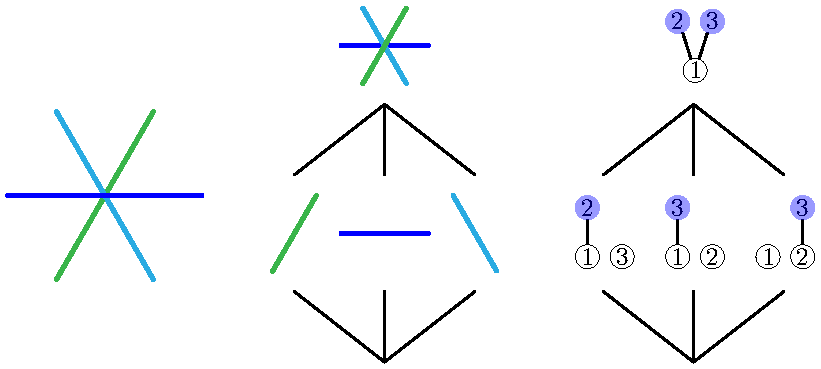
\includegraphics[scale=.9]{figures/intersectionPosetBraidArrangement31Full}}
	\caption{The braid arrangement $\braidArrangement[3]$ (left), its flat poset~$\flatPoset[{\braidArrangement[3]}]$ (middle), and its interpretation in terms of forests (right).}
	\label{fig:braidArrangement31}
\end{figure}

\begin{figure}
	\centerline{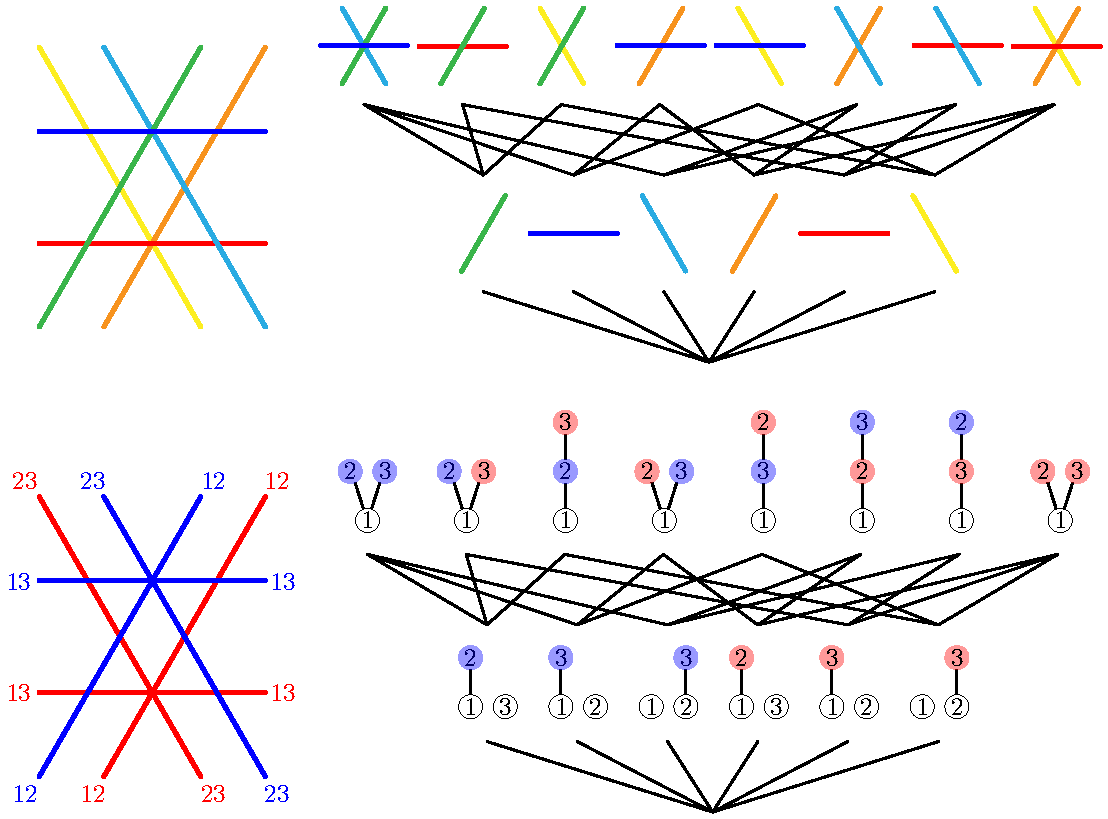
\includegraphics[scale=.9]{figures/intersectionPosetBraidArrangement32Full}}
	\caption{The $(2,3)$-braid arrangement $\lBraidArrangement[3][2]$ (left), its flat poset~$\flatPoset[{\lBraidArrangement[3][2]}]$ (top right), and its interpretation in terms of colored forests (bottom right).}
	\label{fig:braidArrangement32}
\end{figure}

\begin{definition}
The \defn{intersection hypergraph}~$I(F_1, \dots, F_\ell)$ of a $\ell$-tuple of partitions of~$[n]$ is the $\ell$-regular $\ell$-partite hypergraph on all parts of all the partitions~$F_i$, with an hyperedge for all~$i \in [n]$ connecting the parts containing~$i$.
A \defn{$(\ell,n)$-forest} (resp.~\defn{$(\ell,n)$-tree}) is a $\ell$-tuple~$\b{F} \eqdef (F_1, \dots, F_\ell)$ of partitions of~$[n]$ whose intersection hypergraph is a hyperforest (resp.~hypertree).
See \cref{fig:forests}.
The \defn{$(\ell,n)$-forest poset} is the poset~$\forestPoset$ on $(\ell,n)$-forests ordered by componentwise refinement.
In other words, $\forestPoset$ is the subposet of the $\ell$th Cartesian power of the partition poset~$\partitionPoset$ induced by $(\ell,n)$-forests.
Note that the maximal elements of~$\forestPoset$ are the $(\ell, n)$-trees.
%
\begin{figure}
	\centerline{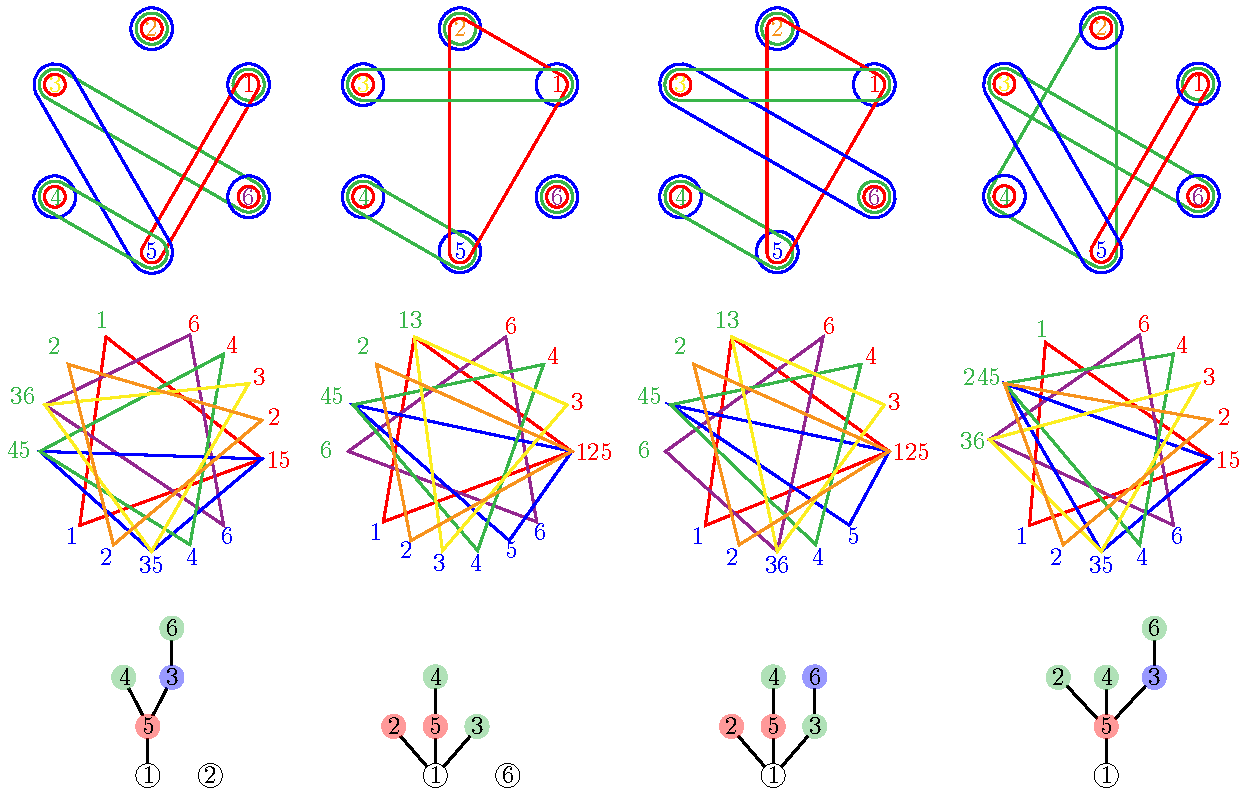
\includegraphics[scale=.9]{forests}}
	\caption{A $(3,6)$-forest with its intersection hypergraph and the corresponding forest (top) and a $(3,6)$-tree with its intersection hypertree and the corresponding tree (bottom).}
	\label{fig:forests}
\end{figure}
\end{definition}



\begin{definition}
A \defn{$(\ell,n)$-colored forest} (resp.~\defn{$(\ell,n)$-colored tree}) is a rooted forest whose nodes are labeled (bijectively) by~$[n]$ and properly (no monochromatic edge) colored by~$\{0,\dots,n\}$ such that the roots of the forest are precisely the nodes colored~$0$.
See \cref{fig:forests}.
\end{definition}

%\begin{remark}
%Note that by rooting each connected component of the $(\ell,n)$ forest in its smallest label and splitting hyperedges in edges between each vertex of the hyperedge and the closest vertex from the root one get the following alternative definitions for  $(\ell,n)$-forests and  $(\ell,n)$-trees:
%A {$(\ell,n)$-forest} (resp.~{$(\ell,n)$-tree}) is a forest (resp. tree) in which:
%\begin{itemize}
%\item each root is the smallest in its connected component 
%\item edges are colored by $\{1, \ldots, \ell\}$ 
%\item if a vertex $v$ is not a root, the unique path from $v$ to the root starts with an edge $e$ of color $c$: $e$ is then the only edge adjacent to $v$ of this color. 
%\end{itemize}
%We represent this interpretation of $(\ell,n)$-forests on Figure \ref{fig:forests} and the according intersection poset of $\lBraidArrangement[3][2]$ on Figure \ref{fig:braidArrangementTrees32}. 
%\vincent{Retravailler}
%\end{remark}

%\begin{figure}
%	\centerline{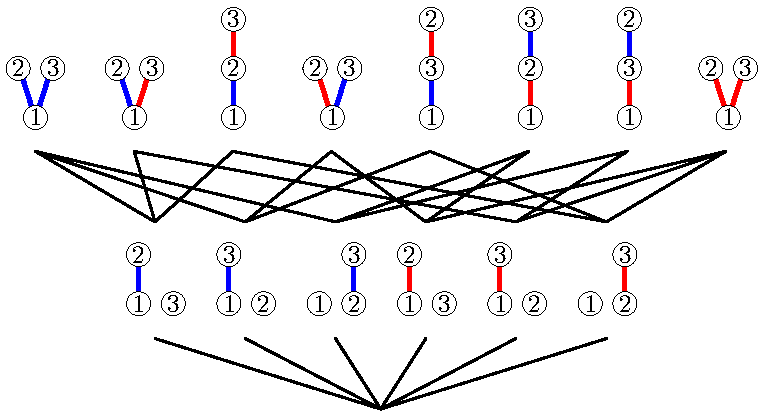
\includegraphics[scale=.9]{figures/intersectionPosetBraidArrangementTrees32}}
%	\caption{The flat poset of $\lBraidArrangement[3][2]$ in terms of forests. See also \cref{fig:braidArrangement32}.}
%	\label{fig:braidArrangementTrees32}
%\end{figure}

\vincent{Explain that the flat poset is given by these forests.}

\begin{theorem}
\label{thm:MobiusPolynomial}
The M\"obius polynomial of the $(\ell,n)$-braid arrangement~$\lBraidArrangement$ is given by
\[
\mobPol[\lBraidArrangement] = x^{n-1-\ell n} y^{n-1-\ell n} \sum_{\b{F} \le \b{G}} \prod_{i \in [\ell]} x^{\#F_i} y^{\#G_i} \prod_{p \in G_i} (-1)^{\#F_i[p]-1} (\# F_i[p]-1)! \; ,
\]
where~$\b{F} \le \b{G}$ ranges over all intervals of the $(\ell,n)$-forest poset~$\forestPoset$, and~$F_i[p]$ denotes the restriction of the partition~$F_i$ to the part~$p$ of~$G_i$.
\end{theorem}

\begin{proof}
Observe that for~$\b{F} = (F_1, \dots, F_\ell)$ and~$\b{G} = (G_1, \dots, G_\ell)$ in~$\forestPoset$, we have
\[
[\b{F}, \b{G}] = \prod_{i \in [\ell]} [F_i, G_i] \simeq \prod_{i \in [\ell]} \prod_{p \in G_i} \partitionPoset[{\#F_i[p]}].
\]
As the M\"obius function is multiplicative, that is,
\(
\mu_{P \times Q} \big( (p,q), (p’,q’) \big) = \mu_P(p,p’) \cdot \mu_Q(q,q’),
\)
we obtain that
\[
\mu_{\forestPoset}(\b{F}, \b{G}) = \prod_{i \in [\ell]} \prod_{p \in G_i} (-1)^{\#F_i[p]-1} (\# F_i[p]-1)!
\]
Hence
\begin{align*}
\mobPol[\lBraidArrangement] 
& = \sum_{\b{F} \le \b{G}} \mu_{\forestPoset}(\b{F}, \b{G}) \, x^{\dim(\b{F})} \, y^{\dim(\b{G})} \\
& = x^{n-1-\ell n} y^{n-1-\ell n} \sum_{\b{F} \le \b{G}} \prod_{i \in [\ell]} x^{\#F_i} y^{\#G_i} \prod_{p \in G_i} (-1)^{\#F_i[p]-1} (\# F_i[p]-1)!.
\qedhere
\end{align*}
\end{proof}

We thus obtain the following statament from \cref{thm:MobiusPolynomial,thm:Zaslavsky}.

\begin{corollary}
\label{coro:fbvectorslBraidArrangement}
The $f$- and $b$-polynomials of the $(\ell,n)$-braid arrangement~$\lBraidArrangement$ are given by
\begin{align*}
\fPol[\lBraidArrangement] & = x^{n-1-\ell n}\sum_{\b{F} \le \b{G}} \prod_{i \in [\ell]} x^{\#F_i} \prod_{p \in G_i} (\# F_i[p]-1)!\\
\text{and}\qquad
\bPol[\lBraidArrangement] & = (-1)^\ell x^{n-1-\ell n} \sum_{\b{F} \le \b{G}} \prod_{i \in [\ell]} x^{\#F_i} \prod_{p \in G_i} -(\# F_i[p]-1)!
\end{align*}
\end{corollary}

The face numbers and bounded face numbers of~$\lBraidArrangement$ for~$\ell, n \in [4]$ are gathered in \cref{table:fvectorlBraidArrangements}.

\begin{example}
For~$n = 1$, we have
\[
\mobPol[{\lBraidArrangement[1][\ell]}] = \fPol[{\lBraidArrangement[1][\ell]}] = \bPol[{\lBraidArrangement[1][\ell]}] = 1.
\]
For~$n = 2$, we have
\[
\mobPol[{\lBraidArrangement[2][\ell]}] = xy-\ell x+\ell,
\quad
\fPol[{\lBraidArrangement[2][\ell]}] = (\ell+1)x+\ell
\quad\text{and}\quad
\bPol[{\lBraidArrangement[2][\ell]}] = (\ell-1)x+\ell.
\]
The case~$n = 3$ is already more interesting.
Consider the partitions~$P \eqdef \big\{ \{1\}, \{2\}, \{3\} \big\}$, $Q_i \eqdef \big\{ \{i\}, [3] \ssm \{i\} \big\}$, and~$R \eqdef \big\{ [3] \big\}$.
Observe that the $(\ell,3)$-forests are all of the form
\begin{gather*}
\b{F} \eqdef P^\ell,
\quad
\b{G}_i^p \eqdef P^p Q_i P^{\ell-p-1}, % \text{ for } p \le \ell-1 \text{ and } i \in [3],
\quad
\b{H}_{i,j}^{p,q} \eqdef P^p Q_i P^{\ell-p-q-2} Q_j P^q \;\text{($i \ne j$)} % \text{ for } p + q \le \ell-2 \text{ and } i \ne j \in [3]
\quad\text{or}\quad
\b{K}^p \eqdef P^p R P^{\ell-p-1}. % \text{ for } p \le \ell-1.
\end{gather*}
(where we write a tuple of partitions of~$[3]$ as a word on~$\{P, Q_i, R\}$, and $p$ and $q$ are such that the total length is~$\ell$).
%\begin{gather*}
%\b{F} \eqdef (\underbrace{P, \dots, P}_\ell), \\
%\b{G}_i^p \eqdef (\underbrace{P, \dots, P}_p, Q_i, \underbrace{P, \dots, P}_{\ell-p-1}) \text{ for } p \le \ell-1 \text{ and } i \in [3],
%\\
%\b{H}_{i,j}^{p,q} \eqdef (\underbrace{P, \dots, P}_p, Q_i, \underbrace{P, \dots, P}_{\ell-p-q-2}, Q_j, \underbrace{P, \dots, P}_q) \text{ for } p + q \le \ell-2 \text{ and } i \ne j \in [3],
%\\
%\text{or}\quad
%\b{K}^p \eqdef (\underbrace{P, \dots, P}_p, R, \underbrace{P, \dots, P}_{\ell-p-1}) \text{ for } p \le \ell-1.
%\end{gather*}
Moreover, the cover relations in the $(\ell,3)$-forest poset are precisely the relations
%\[
%\b{F} \le \b{G}_i^p \begin{array}{c@{\hspace{-.3cm}}c@{\hspace{-.3cm}}c} & \b{H}_{i,j}^{p,q} & \\ \rotatebox[origin=c]{45}{$\le$} & & \rotatebox[origin=c]{-45}{$\le$} \\[.3cm] \rotatebox[origin=c]{-45}{$\le$} & & \rotatebox[origin=c]{45}{$\le$} \\ & \b{H}_{j,i}^{\ell-q-1, \ell-p-1} & \end{array} \b{K}^p
%\]
\[
\b{F} \le \b{G}_i^p \hspace{-.4cm} \begin{array}{l} \rotatebox[origin=c]{45}{$\le$} \raisebox{.2cm}{$\b{H}_{i,j}^{p,q}$} \\[.1cm] \quad \le \b{K}^p \\[.1cm] \rotatebox[origin=c]{-45}{$\le$} \raisebox{-.2cm}{$\b{H}_{j,i}^{\ell-q-1, \ell-p-1}$} \end{array}
\]
for~$i \ne j$ and~$p, q$ such that~$p + q \le \ell-2$.
Hence, we have
\begin{align*}
\mobPol[{\lBraidArrangement[3][\ell]}] & = x^2 y^2 - 3 \ell x^2 y + \ell (3 \ell - 1) x^2 + 3 \ell x y - 3 \ell (2 \ell - 1) x + \ell (3 \ell - 2) , \\
\fPol[{\lBraidArrangement[3][\ell]}] & = (3 \ell^2 + 2 \ell + 1) x^2 + 6 \ell^2 x + \ell (3 \ell - 2), \\
\text{and}\qquad
\bPol[{\lBraidArrangement[3][\ell]}] & = (3 \ell^2 - 4 \ell + 1) x^2 + 6 \ell (\ell - 1) x + \ell (3 \ell - 2).
\end{align*}
Note that~$3 \ell^2 + 2 \ell + 1$ is~\OEIS{A056109}, that~$\ell (3 \ell - 2)$ is~\OEIS{A000567}, and that~$3 \ell^2 - 4 \ell + 1$ is~\OEIS{A045944}.
\vincent{There is a weird connection between the first and the last. Namely, $3 \ell^2 - 4 \ell + 1 = 3 (\ell - 1)^2 + 2 (\ell - 1)$. Is there a bijective explanation on the arrangements?}
\end{example}

\begin{theorem}
\label{thm:verticeslnBraidArrangement}
The number of vertices of the $(\ell,n)$-braid arrangement~$\lBraidArrangement$ (or equivalently of $(\ell,n)$-trees) is
\[
f_0(\lBraidArrangement) = \ell \big( (\ell-1) n + 1)^{n-2}.
\]
\end{theorem}

\begin{proof}
We adapt the proof from \cite{CKSS04}. By rooting in the part of colour $1$ containing $1$, the number of vertices of the $(\ell,n)$-braid arrangement~$\lBraidArrangement$ is the same as the number of Cayley trees rooted in $1$ with an edge-coloring by $\{1, \ldots, \ell\}$ satisfying that the colour of an edge from a child is different from the colour of the edge between the parent and the child. A common reasoning for counting Cayley trees is the use of its Prüfer code defined by recursively pruning the smallest leaf and writing down the number of its parent. This bijection can be adapted to edge-coloured Cayley trees by writing down the number of the parent and the colour of the edge linking the leaf to its parent. We get a coloured word of length $n-1$. Their are two possibilities:
\begin{itemize}
\item either the node we are removing is attached to the root labelled by $1$ and there are $\ell$ possible different colours for the edge ($\ell$)
\item or it is attached to one of the $n-1$ other nodes and the edge can have $\ell-1$ different colours. ($(n-1)(\ell-1)$)
\end{itemize}
 Note that the last letter in the Prüfer code (obtained by removing the last edge) is necessarily the root $1$, with $\ell$ possible different colours.
 There are $(\ell+(n-1)(\ell-1))^{n-2} \times \ell$ such words, hence the result.
\end{proof}

\begin{conjecture}
\label{thm:verticesRefinedlnBraidArrangement}
For any~$k_1, \dots, k_\ell$ such that~$0 \le k_i \le n-1$ for all~$i \in [\ell]$ and~$\sum_{i=1}^\ell k_i = n-1$, the number of vertices~$v$ of the $(\ell,n)$-braid arrangement~$\lBraidArrangement$ such that the smallest flat of the $i$th copy of~$\braidArrangement$ containing~$v$ has dimension~$n-k_i-1$ is given by
\[
n^{\ell-1}  \binom{n-1}{k_1, ..., k_\ell} \prod_{i=1}^\ell (n-k_i)^{k_i-1}.
\]
\end{conjecture}


\vincent{TODO: Check whether we can say something on the facets as well. I guess not, but I want to be sure.}

\vincent{TODO: Discuss generalizations to $\ell$ copies of an arbitrary arrangement, or a graphical arrangement.}

\subsection{Enumerative results for any diagonal} 
\label{s:facets}

We now specialize the results of the previous section to the case~$\ell = 2$ to derive enumerative results on the diagonal of the permutahedron.

Note that
\begin{align*}
\mobPol[{\lBraidArrangement[1][2]}] & = 1 \\
\mobPol[{\lBraidArrangement[2][2]}] & = x y - 2 x + 2 \\
\mobPol[{\lBraidArrangement[3][2]}] & = x^2 y^2 - 6 x^2 y + 10 x^2 + 6 x y - 18 x + 8 \\
\mobPol[{\lBraidArrangement[4][2]}] & = x^3 y^3 - 12 x^3 y^2 + 52 x^3 y - 84 x^3 + 12 x^2 y^2 - 96 x^2 y + 216 x^2 + 44 x y - 182 x + 50 \\
\mobPol[{\lBraidArrangement[5][2]}] & = x^4 y^4 - 20 x^4 y^3 + 160 x^4 y^2 - 620 x^4 y + 1008 x^4 + 20 x^3 y^3 - 300 x^3 y^2 + 1640 x^3 y - 3360 x^3 \\ & \quad+ 140 x^2 y^2 - 1430 x^2 y + 4130 x^2 + 410 x y - 2210 x + 432
\end{align*}
which can be seen on matrices as
\[
\left(\begin{array}{r}
1
\end{array}\right)
\left(\begin{array}{rr}
2 & -2 \\
0 & 1
\end{array}\right)
\left(\begin{array}{rrr}
8 & -18 & 10 \\
0 & 6 & -6 \\
0 & 0 & 1
\end{array}\right)
\left(\begin{array}{rrrr}
50 & -182 & 216 & -84 \\
0 & 44 & -96 & 52 \\
0 & 0 & 12 & -12 \\
0 & 0 & 0 & 1
\end{array}\right)
\left(\begin{array}{rrrrr}
432 & -2210 & 4130 & -3360 & 1008 \\
0 & 410 & -1430 & 1640 & -620 \\
0 & 0 & 140 & -300 & 160 \\
0 & 0 & 0 & 20 & -20 \\
0 & 0 & 0 & 0 & 1
\end{array}\right)
%\left(\begin{array}{r}
%1
%\end{array}\right)
%\left(\begin{array}{rr}
%2 & 0 \\
%-2 & 1
%\end{array}\right)
%\left(\begin{array}{rrr}
%8 & 0 & 0 \\
%-18 & 6 & 0 \\
%10 & -6 & 1
%\end{array}\right)
%\left(\begin{array}{rrrr}
%50 & 0 & 0 & 0 \\
%-182 & 44 & 0 & 0 \\
%216 & -96 & 12 & 0 \\
%-84 & 52 & -12 & 1
%\end{array}\right)
%\left(\begin{array}{rrrrr}
%432 & 0 & 0 & 0 & 0 \\
%-2210 & 410 & 0 & 0 & 0 \\
%4130 & -1430 & 140 & 0 & 0 \\
%-3360 & 1640 & -300 & 20 & 0 \\
%1008 & -620 & 160 & -20 & 1
%\end{array}\right)
%\left(\begin{array}{rrrrrr}
%4802 & 0 & 0 & 0 & 0 & 0 \\
%-31922 & 4732 & 0 & 0 & 0 & 0 \\
%82560 & -23100 & 1830 & 0 & 0 & 0 \\
%-104400 & 41560 & -6210 & 340 & 0 & 0 \\
%64800 & -32760 & 6960 & -720 & 30 & 0 \\
%-15840 & 9568 & -2580 & 380 & -30 & 1
%\end{array}\right)
\]

\begin{theorem}
\label{thm:vertices2nBraidArrangement}
There are bijections between
\begin{itemize}
\item the vertices of the $(2,n)$-braid arrangement~$\lBraidArrangement[n][2]$,
\item the $(2,n)$-trees (\ie pairs of partitions whose intersection graph is a tree),
\item the spanning trees of the complete graph~$K_{n+1}$ on~$\{0, \dots, n\}$ containing the edge~$(0,1)$.
\end{itemize}
These sets are counted by
\[
f_0(\lBraidArrangement[n][2]) = 2 (n + 1)^{n-2}.
\]
\end{theorem}

\begin{proof}
Note that the formula follows from \cref{thm:verticeslnBraidArrangement}.
We give an alternative simple proof.
The first two sets are in bijection by \cref{coro:fbvectorslBraidArrangement}.
Consider now a $(2,n)$-tree~$\b{F} \eqdef (F_1,F_2)$ (hence~$\# F_1 + \# F_2 = n + 1$).
Consider the intersection tree~$T$ of~$\b{F}$ with vertices labeled by the parts of~$F_1$ and of~$F_2$ and edges labeled by~$[n]$, root~$T$ at the part of~$F_1$ containing vertex~$1$, forget the vertex labels of~$T$, and send each edge label of~$T$ to the next vertex away from the root, and label the root by~$0$.
See \cref{fig:tree}.
The result is a spanning tree of the complete graph~$K_{n+1}$ on~$\{0, \dots, n\}$ which must contain the edge~$(0,1)$ (because we have chosen the root to be the part of~$F_1$ containing~$1$).
%
\begin{figure}
	\centerline{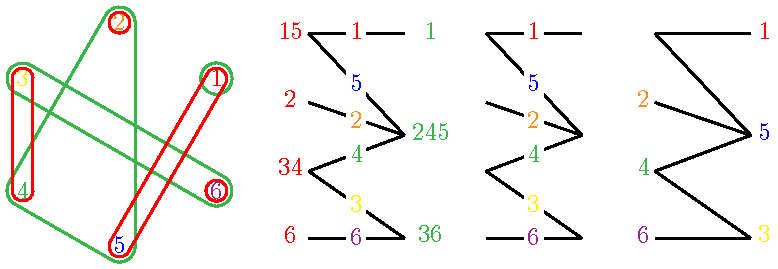
\includegraphics[scale=1]{tree}}
	\caption{The bijection from rooted $(\ell,n)$-trees (left) to spanning trees of~$K_{n+1}$ containing the edge~$(0,1)$ (right).}
	\label{fig:tree}
\end{figure}
%
Finally, by double counting the pairs~$(T,e)$ where $T$ is a spanning tree of~$K_{n+1}$ and $e$ is an edge of~$T$, we see that $n$ times the number of spanning trees of~$K_{n+1}$ equals $\binom{n+1}{2}$ times the number of spanning trees of~$K_{n+1}$ containing~$(0,1)$.
Hence, by Cayley's formula for spanning trees of~$K_{n+1}$, we obtain that
\[
f_0(\lBraidArrangement[n][2]) = \frac{2n}{n(n+1)} (n+1)^{n-1} = 2 (n + 1)^{n-2}.
\qedhere
\]
\end{proof}

\begin{theorem}
\label{thm:verticesRefined2BraidArrangement}
For any~$0 \le k_1, k_2 \le n-1$ with~$k_1 + k_2 = n-1$, the number of vertices~$v$ of the $(2,n)$-braid arrangement~$\lBraidArrangement[n][2]$ obtained as the intersection of a $(n-k_1-1)$-flat of the first copy of the braid arrangement with a $(n-k_2-1)$-flat of the second copy of the braid arrangement is
\[
n \binom{n-1}{k_1} (n-k_1)^{k_1-1} (n-k_2)^{k_2-1}.
\]
\end{theorem}

\begin{proof}
%Note that the formula follows from \cref{thm:verticesRefinedlnBraidArrangement}.
%We give an alternative simple proof.
By \cref{coro:fbvectorslBraidArrangement}, we want to count the number~$t_{k_1,k_2}$ of $(2,n)$-trees~$\b{F} \eqdef (F_1,F_2)$ where~$F_1$ has $n-k_1$ parts while $F_2$ has $n-k_2$ parts.
Consider the intersection tree~$T$ of~$\b{F}$ with vertices labeled by the parts of~$F_1$ and of~$F_2$ and edges labeled by~$[n]$, root~$T$ at an arbitrary part of~$F_1$, forget the vertex labels of~$T$, and send each edge label of~$T$ to the next vertex away from the root.
See \cref{fig:tree}.
Note here that in contrast to the proof of \cref{thm:vertices2nBraidArrangement}, we have rooted~$T$ here at an arbitrary part of~$F_1$ to have more symmetry.
The result is a spanning tree of the complete bipartite graph~$K_{n-k_1, n-k_2}$ together with a choice of which of the labels are on each part of this graph.
Since the number of spanning trees of~$K_{n-k_1, n-k_2}$ is known to be~$(n-k_1)^{n-k_2-1} (n-k_2)^{n-k_1-1} = (n-k_1)^{k_1} (n-k_2)^{k_2}$, we obtain that the number~$t_{k_1,k_2}$ is given by
\[
t_{k_1,k_2} = \underbrace{\frac{1}{n-k_1}  \phantom{\!\!\!\!\bigg)}}_{\text{root}} \underbrace{\binom{n}{n-k_1-1}}_{\text{labels}} \underbrace{(n-k_1)^{k_1} (n-k_2)^{k_2} \phantom{\!\!\!\!\bigg)}}_{\# \text{ spanning trees }} = n \binom{n-1}{k_1} (n-k_1)^{k_1-1} (n-k_2)^{k_2-1}.
\qedhere
\]
\end{proof}

\vincent{Do we want to mention here the refinement counting spanning trees of~$K_{n+1}$ containing~$(0,1)$ according to their number of nodes at even distance from the root?}

\begin{theorem}
\label{thm:facets2BraidArrangement}
The coefficient of~$x^{n-1}$ in the M\"obius polynomial~$\mobPol[{\lBraidArrangement[n][2]}]$ of the $(2,n)$-braid arrangement~$\lBraidArrangement[n][2]$ is given by
\[
[x^{n-1}] \, \mobPol[{\lBraidArrangement[n][2]}] = \frac{(-1)^n n!}{y} \, [z^n] \, \exp \bigg( \sum_{m \ge 1} \frac{- C_m \, y \, z^m}{m} \bigg).
\]
where~$\displaystyle C_m \eqdef \frac{1}{m+1} \binom{2m}{m}$ denotes the $m$th Catalan number.
\end{theorem}

\begin{proof}
We prove that the exponential generating function of the coefficient of~$x^{n-1}$ in the M\"obius polynomial~$\mobPol[{\lBraidArrangement[n][2]}]$ is given by
\[
1 + \sum_{n \ge 1} \frac{[x^{n-1}] \, \mobPol[{\lBraidArrangement[n][2]}] \, y \, z^n}{(n+1)!} = \exp \bigg( \sum_{m \ge 1} \frac{(-1)^{m-1} C_m \, y \, z^m}{m} \bigg).
\]
\vincent{TODO. The proof from my email is in the comments.}
%Consider a forest of cliques F. Each connected component K is a tree of cliques. Consider the labeled intersection tree of this tree of cliques (whose nodes are the cliques and whose edges are the intersections of cliques, labeled by unique element in the intersection). As the clique corresponding to each node of this intersection tree is just formed by the labels of the edges incident to it, we can forget the cliques inside the nodes and just remember the labels on the edges. Now root K on the node corresponding to the clique of F_0 containing the smallest element of K, orient all edges towards this root, order the incoming edges at each node by their labels. You get a rooted planar tree, with some labels on the edges. Consequently, I can see a forest of cliques with c connected as a set of c rooted planar trees whose edges are labeled by [n] (each label appears only once, in only one of the trees), and such that
%	(a) the labels of the edges incoming to a node are well ordered (ie. increasing from the left node to the right node),
%	(b) in each tree, the edge with the smallest label is incident to the root.
%Conversely, I can start from a set of c rooted planar trees, I can label the edges by choosing a permutation of [n], except that 
%	(a) at each node of each of my rooted planar trees, I should divide by the factorial of the incoming degree of my node… this is the (|p|-1)!
%	(b) in each rooted planar tree T, I should divide by the number of edges of my tree to replace the smallest label on an edge incident to the root… this is the /n.
\end{proof}

\begin{corollary}
The numbers of regions and of bounded regions of the $(2,n)$-braid arrangement~$\lBraidArrangement[n][2]$ are given by
\begin{align*}
f_{n-1}(\lBraidArrangement[n][2]) 
& = n! \, [z^n] \exp \bigg( \sum_{m \ge 1} \frac{C_m \, z^m}{m} \bigg) \\
\text{and}\qquad
b_{n-1}(\lBraidArrangement[n][2]) 
% & = - (n+1)! \, [z^{n+1}] \exp \left( - \sum_{m \ge 1} \frac{z^m}{m(m+1)} \binom{2m}{m} \right) 
& = (n-1)! \, [z^{n-1}] \exp \bigg( \sum_{m \ge 1} C_m \, z^m \bigg).
\end{align*}
The corresponding integer sequences are
\begin{align*}
1, 3, 17, 149, 1809, 28399, 550297, 12732873, \dots & \qquad \text{\OEIS{A213507}}, \\
\text{and}\qquad
1, 1, 5, 43, 529, 8501, 169021, 4010455, 110676833, \dots & \qquad \text{\OEIS{A251568}}.
\end{align*}
\vincent{TODO: improve presentation}
\end{corollary}

\begin{proof}
As $\fPol[{\lBraidArrangement[n][2]}] = \mobPol[{\lBraidArrangement[n][2]}][-x][-1]$ and $\bPol[{\lBraidArrangement[n][2]}] = \mobPol[{\lBraidArrangement[n][2]}][-x][1]$ by \cref{thm:Zaslavsky}, we obtain from \cref{thm:facets2BraidArrangement} that
\begin{align*}
f_{n-1}(\lBraidArrangement[n][2]) & = [x^{n-1}] \, \fPol[{\lBraidArrangement[n][2]}] = (-1)^{n-1} \, [x^{n-1}] \, \mobPol[{\lBraidArrangement[n][2]}][-x][-1] = n! \, [z^n]  \, \exp \bigg( \sum_{m \ge 1} \frac{C_m \, z^m}{m} \bigg), \\
% \text{and}\qquad
b_{n-1}(\lBraidArrangement[n][2]) & = [x^{n-1}] \, \bPol[{\lBraidArrangement[n][2]}] = (-1)^{n-1} \, [x^{n-1}] \, \mobPol[{\lBraidArrangement[n][2]}][-x][1] = - n! \, [z^n]  \, \exp \bigg( \sum_{m \ge 1} \frac{- C_m \, z^m}{m} \bigg).
\end{align*}
To conclude, we thus just need to observe that
\(
F(z) = \frac{\partial}{\partial z} G(z)
\)
where
\[
F(z) \eqdef \exp \bigg( \sum_{m \ge 1} C_m \, z^m \bigg)
\qquad\text{and}\qquad
G(z) \eqdef - \exp \bigg( \sum_{m \ge 1} \frac{- C_m \, z^m}{m} \bigg).
\]
For this, consider the generating functions
\[
C(z) \eqdef \sum_{m \ge 0} C_m \, z^m
\qquad\text{and}\qquad
D(z) \eqdef \sum_{m \ge 1} \frac{C_m \, z^m}{m}.
\]
Recall that~$C(z)$ satisfies the functional equation~$C(z) = 1 + z \, C(z)^2$.
We thus obtain that~$C'(z) \big( 1 - 2 \, z \, C(z) \big) = C(z)^2$ and $C(z) \big( 1 - 2 \, z \, C(z) \big) = 2 - C(z)$.
Combining these two equations, we get
\begin{equation}
\label{eq:diff}
C(z)^3 = C'(z) \big( 1 - C(z) \big).
\end{equation}
Observe now that $z \, D'(z) = C(z) - 1 = z \, C(z)^2$, so that~$D''(z) = 2 \, C(z) \, C'(z)$.
Hence
\[
F(z) = \exp \big( C(z) - 1 \big) = \exp \big( z \, D’(z) \big)
\]
and
\[
\frac{\partial}{\partial z} G(z) = \frac{\partial}{\partial z}  - \exp \big( -D(z) \big) = D'(z) \exp \big( -D(z) \big)
\]
Consider the function
\[
H(z) = G'(z) / F(z) = D'(z) \exp \big( -D(z) - z \, D'(z) \big).
\]
Clearly, $H(0) = 1$ and its derivative is
\begin{align*}
H'(z)
& = \Big( D''(z) \big(1 - z \, D'(z) \big) - 2 D'(z)^2 \Big) \exp \big( -D(z) - z \, D'(z) \big) \\
& = 2 \, C(z) \Big( C'(z) \big( 2 - C(z) \big) - C(z)^3 \Big) \exp \big( - D(z) - z \, D'(z) \big),
\end{align*}
which vanishes by~\eqref{eq:diff}.

\vincent{Can we make a bijective proof of the equality $F(z) = \frac{\partial}{\partial z} G(z)$?}
\end{proof}

